\section{各向异性弥散与波场偏移精度}
\label{sec:4.2}

波场偏移时形成两种截然不同类型的误差,属于有较大实际重要性者为频散,它出现在
不同频率成分以不同速度传播的时候。改善有限差分近似对微分的精度,能够减小这类误差,
办法就是加密差分网格;参阅\ref{sec:4.3}节,具有次要重要性且为本节讨论主题的误差,是各向异性
弥散(anisotropy dispersion)。各向异性的波动传播就是波沿不同方向以不同速度行进。

原则上,各向异性弥散可用Muir平方根展开式来补救。实际上,展开一般是按15°项或
者45°项来截断的,形成了数据处理中的各向异性误差。为截断级数因而不惜引起误差的理
由往往是:(1)处理的时间耗费;(2)在总的数据采集与处理的活动中,有其他大量误
差,相比之下,不算什么。为了

(1)在问题出现时能够认识它;

(2)理解在时间耗费和精确度之间采取基本的折衷办法。

应当认真研究各向异性误差这个问题。

各向异性经常同光在晶体中的传播有关。在反射地震学中,各向异性有时涉及到要正确
解释井中速度观测(垂直传播)与用正常时差校正所确定的速度(水平传播)二者之间的细
微差别。这些基本的性质,即物理的各向异性和作为本节主题之数据处理中的各向异性,具
有共同的数学基础和概念基础。



\subsection{不垂直于波阵面的射线}
\label{sec:4.2.1}

各向异性的意思是指,沿不同方向传播的波各以不同速度传播。各向异性并不意味着速
度是空间位置的函数,因而各向异性并不引起射线弯曲。有关各向异性的独有现象是,射线
不垂直于波阵面,可用图\ref{fig:dspr/aniso}说明这种思想。该图的左图表示由位于原点的点震源发射出
的球形波阵面,这就是通常说的各向同性情形。右图表示15°偏移方程的非球形波阵面,注
意,它们在接近$z$轴处是近乎球形波阵面的,但是远离该轴时,它们同中心位于原点的球形
就差得远了。

\begin{figure}[H]
\centering
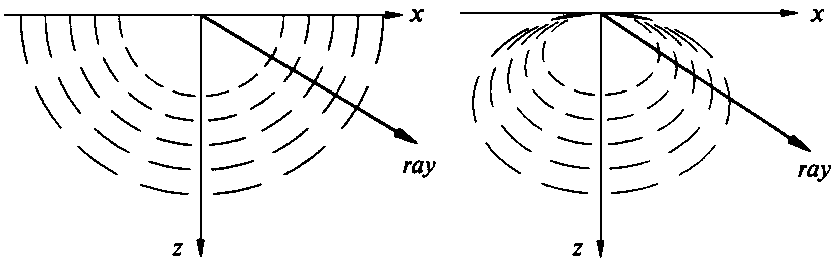
\includegraphics[width=0.65\textwidth]{dspr/aniso}
\caption[aniso]{各向同性介质中的波阵面(左图)及各向异性介质中的波阵面(右图)。注意,
在右图中,涉嫌均不垂直于波阵面(据Rothman)}
\label{fig:dspr/aniso}
\end{figure}

惠更斯二次震源所形成的理想波阵面应是一个半圆。由15°外推方程形成的二次震源波
阵面应是椭圆;由45°外推方程形成的二次震源波阵面是一种有趣的心脏形,这些均绘于图
图\ref{fig:dspr/anisoxz}
内。实际上,棉圆与心脏形之顶部很少能被看
到,因为它们均位于指数衰减区域之内,而且沿欠轴
的点距极少可能加密到足以显示它们所需的低于空间假
频的程度。采用45°外推程序时,有时能在$(x,t)$平
面内看出该心脏形曲线的中心,图\ref{fig:dspr/anisoxt}中所绘直线即
用以表示该中心。采闱45°绕射程序处理时的情形如图\ref{fig:dspr/45imp}所示。

\begin{figure}[H]
\centering
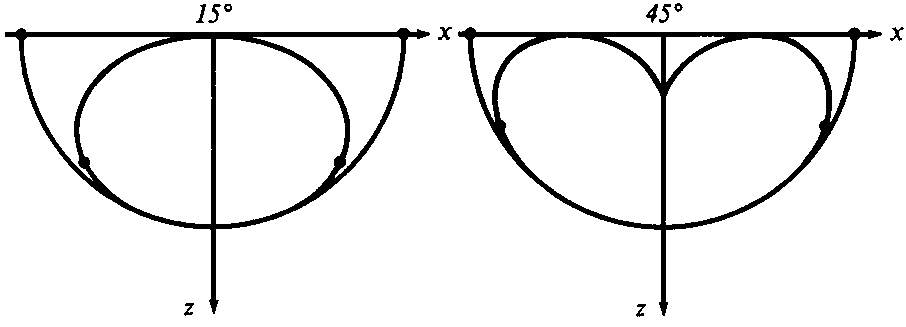
\includegraphics[width=0.65\textwidth]{dspr/anisoxz}
\caption[anisoxz]{15°外推方程的波阵面(左图)及45°外推方程的波阵面(右图),二者均内接于半圆之内。
凡属$\frac{vk_x}{\omega}=\sin\theta=\pm1$的波均以小黑点表示,倏逝波均在曲线脱离半圆之处的小圆点
以上(据Rothman)}
\label{fig:dspr/anisoxz}
\end{figure}

\begin{figure}[H]
\centering
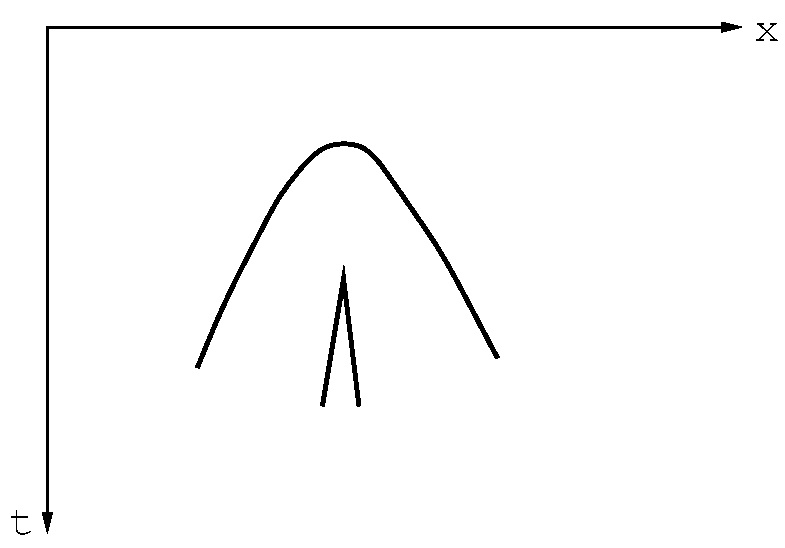
\includegraphics[width=0.65\textwidth]{dspr/anisoxt}
\caption[anisoxt]{45°外推方程的心脏形理论曲线。尖点
出现在指数衰减区域内(据Rothman)}
\label{fig:dspr/anisoxt}
\end{figure}

\subsection{波阵面方向与能量速度}
\label{sec:4.2.2}

在普通的波动传播理论中,能量传播方向是垂直于
波阵面的。当存在有各向异性弥散时,角度将不再是呈直角了。

\begin{figure}[H]
\centering
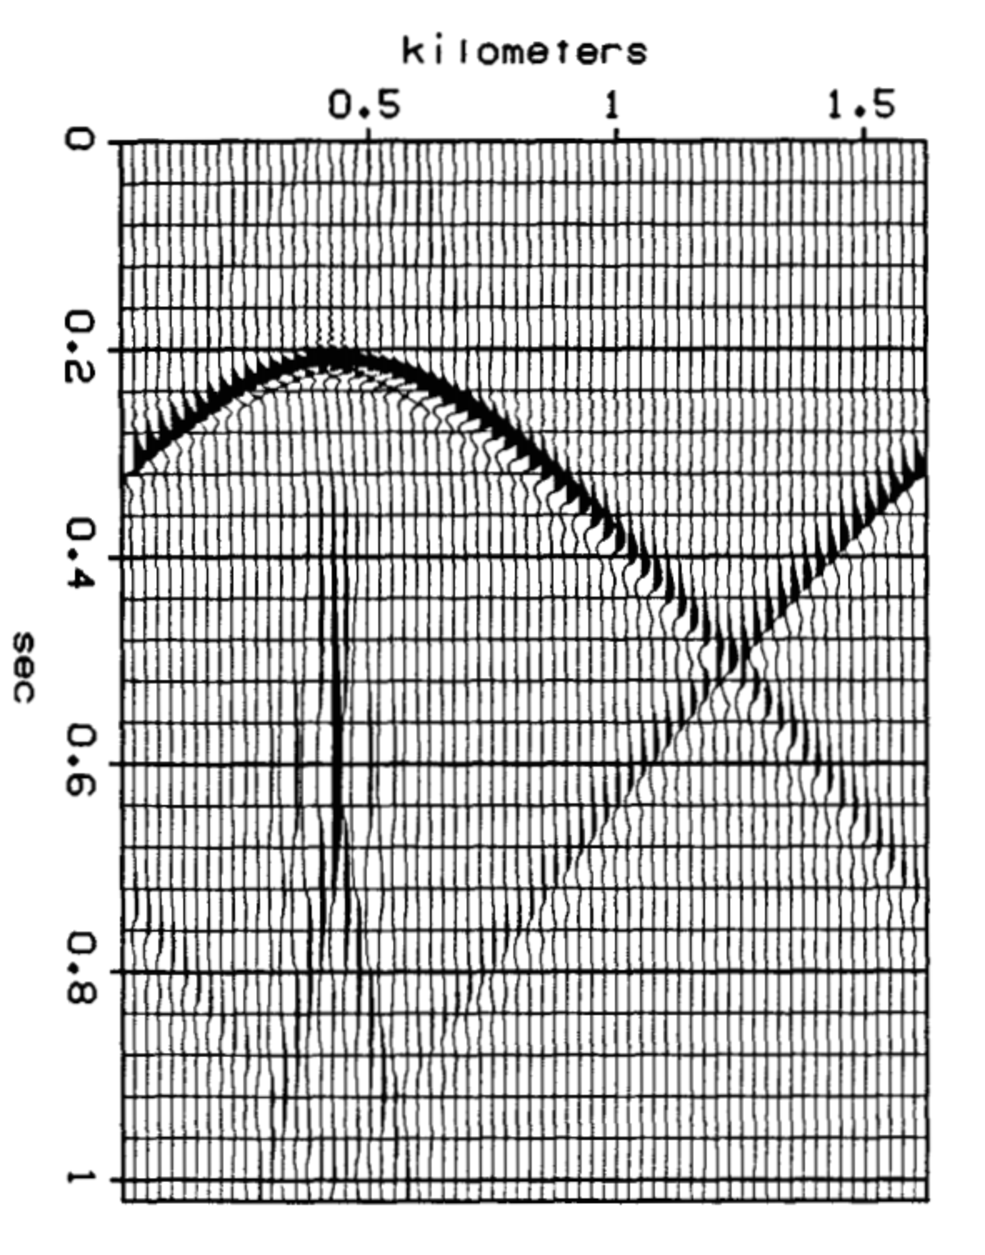
\includegraphics[width=0.65\textwidth]{dspr/45imp}
\caption[45imp]{45°波场外推方程的脉冲响应。$t_0$时间
以前的初至是折叠频率产生的影响。}
\label{fig:dspr/45imp}
\end{figure}

沿地表能看到的水平视速度为$dx/dt$,沿垂直方向
的视速度(如在井中所见)为$dz/dt$,根据几何关系可
知,这些视速度全都大于波动传播速度。大小与速度呈
反比而方向垂直于波阵面的一个向量,称作慢度向量
\begin{equation*}
\text{慢度向量}=(\frac{dt}{dx},\frac{dt}{dz})
\end{equation*}
沿慢度向量的方向行进但具有波阵面法线速度的一种向
量,定义为相速度向量,更精确地说,相速度向量等于慢度向量除以其平方幅度
\begin{equation*}
\text{相速度}=\frac{(\frac{dt}{dx},\frac{dt}{dz})}{(\frac{dt}{dx})^2+(\frac{dt}{dz})^2}
\end{equation*}

就正弦形扰动$\exp(i\phi)=\exp(-i\omega t+ik_xx+ik_zz)$
而言,可令相位$\phi$等于常数
\begin{equation*}
d\phi=-\omega dt+k_xdx+k_zdz=0
\end{equation*}
因而,在Fourier空间内,慢度向量为
\begin{subequations}
\begin{equation}
\text{慢度向量}=(\frac{k_x}{\omega},\frac{k_z}{\omega})
\label{eq:ex4.2.1a}
\end{equation}
要导出能量传播方向则更为困难一点,不过可由所谓群速度向量导出它
\begin{equation}
\text{群速度向量}=(\frac{\partial}{\k_x},\frac{\partial }{k_z})\omega(k_x,k_z)
\label{eq:ex4.2.1b}
\end{equation}
\end{subequations}
对于标量波动方程应有$\omega^2/v^2=k_x^2+k_z^2$,由是迸行微分并代入,可以证明群速度向量原来同
相速度向量是相同的。最熟悉的弥散类型是频散,这时不同频率是以不同速度传播。以后本
节将会指出,熟悉的外推方程(15°的,45°的等等)并不表现出频散性质。那就是说,作为
$\omega$与角度$k_x/\omega$的函数,在这些方程中的速度并不依赖于频率$\omega$。换句话说,图\ref{fig:dspr/anisoxz}中的椭圆形与心脏形曲线均与频率无关。

各向异性弥散的一个有趣现象是,能量看起来好像是沿某一个方向在行进着而其实它实
际上是在沿另一个方向行进着。当群速度有一个向下分量而相速度有一向上分量时,就会出现
这种现象。描述45°外推方程之弥散关系的图\ref{fig:dspr/group15}就是一个例子,从原点至弥散曲线所画之
箭头表示沿波阵面法线方向的慢度向量,注意到群速度以式\ref{eq:ex4.2.1b}中的梯度算子来每
义,现在就能用图解方法确定相应的群速度方向。试将$\omega$值考虑为一个小山的高度,$k_z$就是
从该$\omega$山头指向南而$k_x$则指向东,于是,弥散关系曲线就是等高线,按不同的比例标度绘出图
\ref{fig:dspr/group15}就形成了不同频率的数值,沿梯度方向的群速度则是垂直于各$\omega$的等值线。

采用活动电影形式可以非常清楚地识别出各向异性弥散现象,尽管在如图\ref{fig:dspr/prism}所示的
单个画面上也可以认识出来。图\ref{fig:dspr/prism}中所绘直线是解释能量由顶部进入,经过棱镜,在棱
镜的45°淘度一侧反射,再从画面的一侧反射,最后进入图中某一个区域,该区域有足够的
大小,因而许多波阵面不致群集一起,足以识别出能量看似向上传播其实真正的是向下传
播。

\begin{figure}[H]
\centering
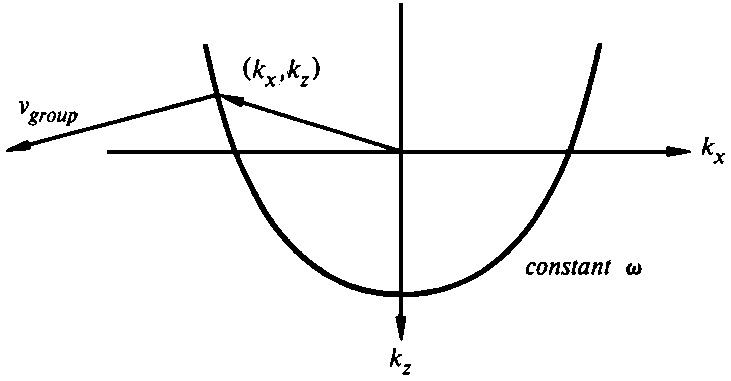
\includegraphics[width=0.65\textwidth]{dspr/group15}
\caption[group15]{表示群速度向量与慢度向量的向下外推方程弥散关系曲线(据Rothman)}
\label{fig:dspr/group15}
\end{figure}

\begin{figure}[H]
\centering
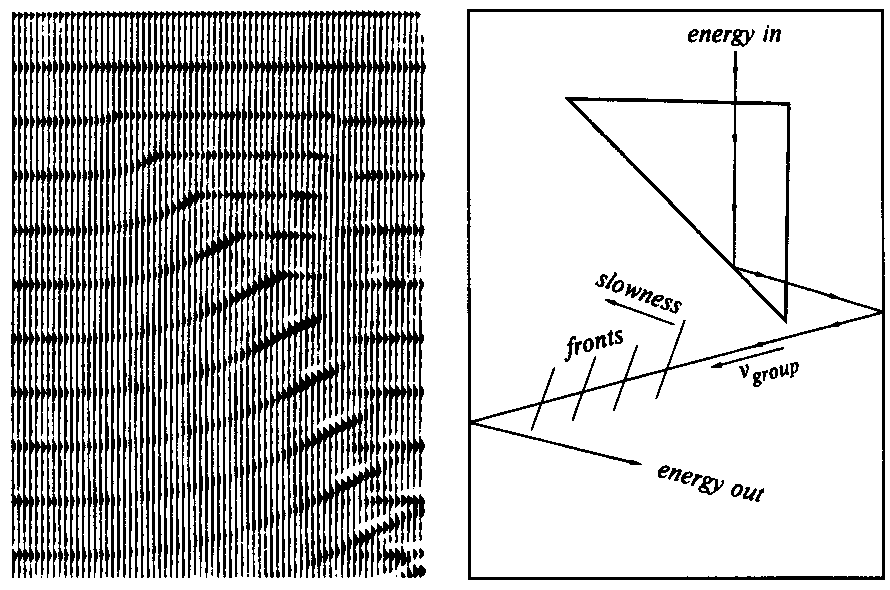
\includegraphics[width=0.65\textwidth]{dspr/prism}
\caption[prism]{四种不同频率的平面波,传播通过一个具有$45$°角度的棱镜。左图为
波场,右图是说明能量的不同方向和波阵面法线方向的射线解释图(据Estevez)}
\label{fig:dspr/prism}
\end{figure}

当你考虑到计算波场所用的程序时,
在图\ref{fig:dspr/prism}中无论能量还是信息都不可能
向上传播,这一点就应更清楚了。程序并
没把整个画面都输入于内存,它每次紧挨着前一个条带,一次计算出一个水平条
带。所以活动电影中的波阵面是貌似向上
移动,似乎很难令人理解。从理论上说,利用45°方程的波场外推方法是不能指望
可以处理达到90°的角度的,而图\ref{fig:dspr/prism}中
的例子却尚表明,虽然是以一种有点不正
常的方式、但确实是可以处理这些极端情形的。

有一次,我在地质上属于是逆掩断层地区的反射地震剖面上观察到过类似的环境条件,
这个剖面目前已不能为我所用,现在大概早就从拥有者的底片中消失了,所以我仅能根据记
忆提供如图\ref{fig:dspr/overthrust}所示的简图。图中,速度随深度而增大,引起射线向上弯曲,并从逆掩断
层的下侧反射。为了想知道在波动方程中究竟正在发生什么事,画出如图\ref{fig:dspr/disper2z}所示的两种不同速度时的弥散曲线,将是很有帮助的。

\begin{figure}[H]
\centering
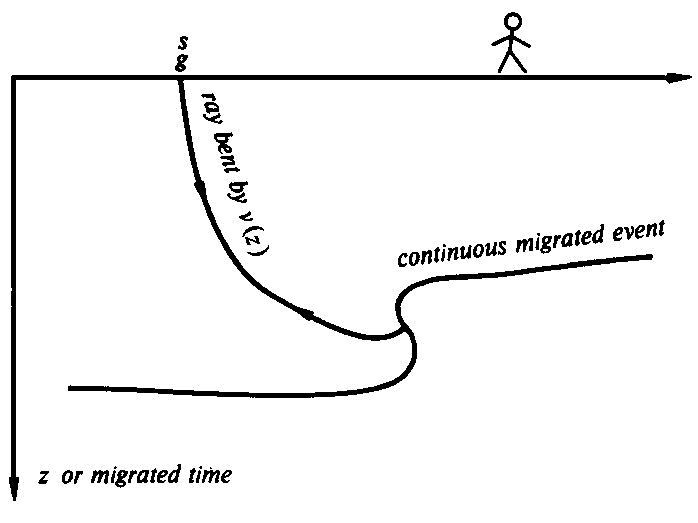
\includegraphics[width=0.65\textwidth]{dspr/overthrust}
\caption[overthrust]{从逆掩断层下侧发生反射的射线}
\label{fig:dspr/overthrust}
\end{figure}

\begin{figure}[H]
\centering
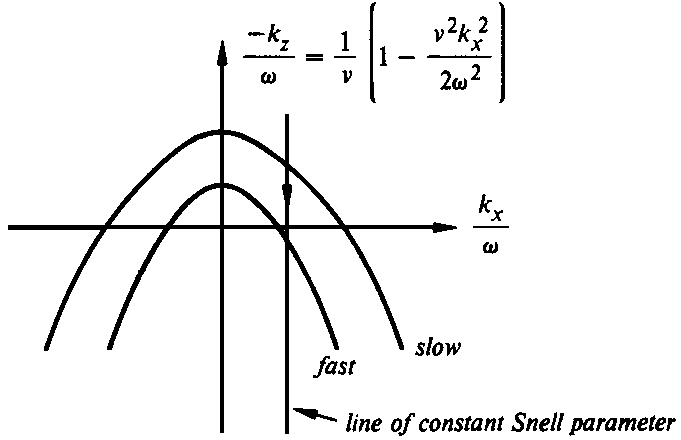
\includegraphics[width=0.65\textwidth]{dspr/disper2z}
\caption[disper2z]{两种不同速度$v_{fast}$与$v_{slow}$时的弥散曲线}
\label{fig:dspr/disper2z}
\end{figure}

具有某种特定时差心的一小部分能量在近地表处(即这时适用低速弥散曲
线)以某种普通的角度开始向下延拓,但是当遇到较深层具有高速的地层时,这时应适用高
速弥散曲线,在此情形下由图\ref{fig:dspr/disper2z}可知,相同的时差$k_x/\omega$却预示着应有负值的相速度。虽
然上冲角的大小未必正确,可总的图象大体是合适的,它很像图\ref{fig:dspr/prism}中所示的情形。如果你想要定量上是正确的偏移,可参阅\ref{sec:4.5}节,或者想要有点完全不同的偏移,则可参阅
Kosloff等(1983)和Baysal等(1983)提出的方法。

\subsection{偏移误差分析}
\label{sec:4.2.3}

利用相速度概念可以对平坦规则的倾斜反射面作整钵分析,仅在同时存在有一个以上的
传播角度时,才需要利用群速度概念。采用点源散射体响应时,会出现这种同时性的要求,
在沿倾斜地层存在有可变反射振幅时,也会出现这种要求。群速度之所以需要,是因为表示
弯曲同相轴或振幅异常,要求平面波传播角度有一定范围。与此类似,在时间序列分析中,
一个经过振輻调制的正弦波之Fourier变换需要有一定频带范围内的正弦谐波。

图\ref{fig:dspr/undermig}所示是光滑平坦倾斜地层,因为用某种有理平方根近似或某种数值近似所定义
的波数$\hat{k_z}$同$k_z$的正确平方根值并不符合一致,以致偏移不足。

\begin{figure}[H]
\centering
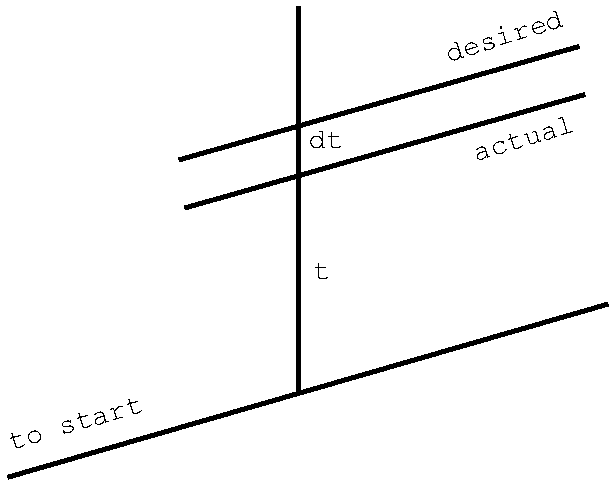
\includegraphics[width=0.65\textwidth]{dspr/undermig}
\caption[undermig]{偏移不足的倾斜反射面}
\label{fig:dspr/undermig}
\end{figure}

图\ref{fig:dspr/undermig}中的误差全部是某种时移误差。由于沿反射面的反射系数为常数,识别不出什
么横向位移误差。该时间误差在理论上可按下式确定:
\begin{equation}
\frac{dt}{t}\approx\frac{dz}{z}\approx\frac{\hat{k_z}-k_z}{k_z}
\label{eq.ex4.2.2}
\end{equation}
就所谓15°外推方程来说,在25°度时所造成的相位误差可证明大约为百分之五十。

其次,我们要确定一下双曲线收缩压扁时的误差。图\ref{fig:dspr/errcollapse}所示是一个双曲线的向下延
拓,为清晰起见,向下延拓没有沿指向聚焦点的所有路径进行。选定某个斜率$p$就可选出具
有某个Snell参量$p=dt/dx$的射线。试想像有一斜率为$p$的切线段切于各双曲线。如果斜率
为p之处有一点振幅异常。那末,你就能在各个双曲面上追踪出它。

\begin{figure}[H]
\centering
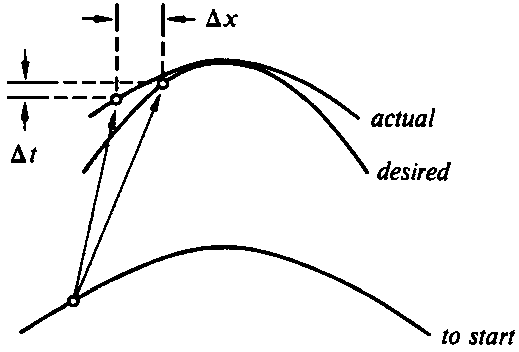
\includegraphics[width=0.65\textwidth]{dspr/errcollapse}
\caption[errcollapse]{双曲线挤缩收敛误差。
注意,实际曲线位于所期望曲线之上,但是
实际的点却是位于所期望点之下}
\label{fig:dspr/errcollapse}
\end{figure}

在图\ref{fig:dspr/errcollapse}中,时间移动量太小了,横向移动距离同样也很小。实际上,具有$r_0=1$的
15°方程的误差,有时采取把深度坐标$z$或者速度$v$增大6\%的办法就能被补偿掉。各误差量可
根据下式计算
\begin{subequations}
\begin{equation}
\frac{\Delta t}{t}=\frac{\frac{\partial}{\partial \omega}(\hat{k_z}-k_z)}{\frac{\partial}{\partial \omega}k_z}
\label{eq:ex4.2.3a}
\end{equation}
\begin{equation}
\frac{\Delta x}{x}=\frac{\frac{\partial}{\partial k_x}(\hat{k_z}-k_z)}{\frac{\partial}{\partial k_x}k_z}
\label{eq:ex4.2.3b}
\end{equation}
\end{subequations}
式中,$k_z$取为$\omega$和$k_x$的函数。它证明,就15°外推方程而言,在角度为20°度时出现百分之五
十左右的群速度误差,因而群速度误差一般是要比相速度误差更为严重的。

\subsection{群速度方程的导出}
\label{sec:4.2.4}
%
% 当速度$v(\omega)$按下述方程定义时
% \begin{equation}
% -\frac{i\omega}{v(\omega)}=\frac{\omega_0}{v_0}(-\frac{i\omega}{\omega_0})^{1-\epsilon}
% \label{eq:ex4.1.3}
% \end{equation}
% 就产生了吸收作用的基本模型。在$\epsilon =
% 0$时,方程\ref{eq:ex4.1.3}给出常速度。在\ref{sec:4.6}节中将证明,
% 方程\ref{eq:ex4.1.3}是模拟所谓的因果性恒定Q值阻尼衰减,此处,$Q^{-1}=\tan \pi\epsilon$。图\ref{fig:dspr/qhale}所示
% 是利用式\ref{eq:ex4.1.2}和\ref{eq:ex4.1.3}按爆炸反射面模型作出的合成地震记录。
%
% \begin{figure}[H]
% \centering
% 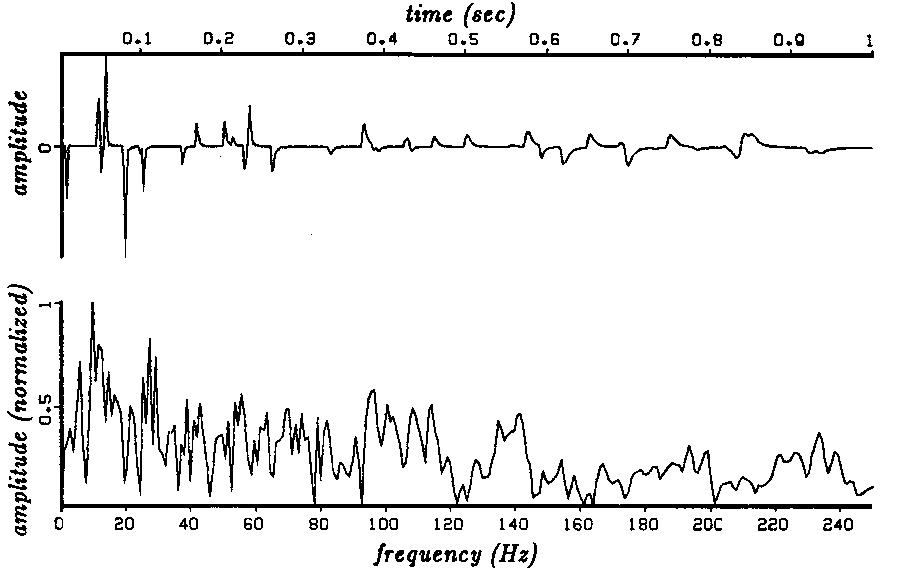
\includegraphics[width=0.65\textwidth]{dspr/qhale}
% \caption[qhale]{地层Q值为$Q=100$时的合成地震记录(据Hale)}
% \label{fig:dspr/qhale}
% \end{figure}
%
% 式\ref{eq:ex4.1.3}在速度中引入了虚部,因而形成衰减,这种衰减的主要影响就是使到达时间
% 晚的初至削弱。第二种影响就是使晚到之初至的频率成分变低。第三种影响则是这样:它之
% 所以出现是由于因果性条件的要求迫使速度的实部或多或少地与频率有关。在图\ref{fig:dspr/qhale}中,
% 各个脉冲的“上升时间”均比“下落时间”(fall
% time)要快,就是证实有这种稍微与频
% 率有关的现象。这种现象意味着高频成分的传播比低频成分稍微快一些。在实际工作中,这
% 第三种影响非常值得注意。
%
% 实现地层成像时,在向下延拓期间放大高频能量,就能够补偿掉地层耗散作用。这种补
% 偿处理除了要以像$ik_z=(-i\omega)^{1-\epsilon}$这种项代替$k_z=\sqrt{k_x^2-\omega^2/v^2}$之外,几乎就能够像偏移一
% 样来完成。不过,由于它会把噪音放大,实际上并没有人愿意这样作。所以,这就产生了信
% 噪比的问题。
%
% 噪音并非简单就是环境背景的随机起伏,如重复放炮,它多半是可重复出现的。噪音是
% 迄今我们还没法提出满意机制模型的一种东西。按照目前的实际处理水平,往往习惯于采用
% 时变滤波来选择中意的时变通带。方程\ref{eq:ex4.1.2}与\ref{eq:ex4.1.3}能够用于实现这种时变滤波,
% 不过要是把它们的使用看成就是补偿地层Q值变化,却是过于简单化了。
%
% \subsection{频散作用}
% \label{sec:4.1.5}
%
% 在有面波存在的情形下,速度对频率的依赖关系是极明显的。例如,速度对频率的依赖
% 关系由下述方程给出
% \begin{equation}
% -\frac{i\omega}{v(\omega)}=-\frac{i\omega}{v_0}\sqrt{1+\omega_0^2/\omega^2}
% \label{eq:ex4.1.4}
% \end{equation}
% 图\ref{fig:dspr/sword}(a)包含有某种频散地滚波。在图\ref{fig:dspr/sword}(b)中,采用类似偏移的处理,该频散现
% 象就消除了。这种处理同偏移处理之间的一种差别就是:偏移是沿$z$轴向下外推,而在图
% \ref{fig:dspr/sword}(b)中则是沿x轴外推(实际上,外推方向都只是在计算机内处理的)。在图\ref{fig:dspr/sword}
% (左图)中,每个记录道都是单独处理。在偏移方法中,利用频散关系$k_z=-\sqrt{\omega^2/v^2-k_x^2}$
% 将数据$p(t,z=0)$外推为映象$p(t=0,z)$;在图\ref{fig:dspr/sword}(左图)的处理中,则是利用像
% $k_x=f(\omega/v)$的这类频散关系将数据$p(t,x=0)$外推为映象$p(t=0,x)$。在完成这种赝偏移
% (pseudomigration)之后,再用常速作廣绕射扫描(pseudodiffraction),其总效果就是
% 消除频散,最终就有可能看出,干扰原来是由两种独立的同相轴组成的。
%
% 类似这样一种处理技术曾经首先应用于探测煤层中的断层(Beresford-Smith与Mas-on, 1980年)。
%
% \begin{figure}[H]
% \centering
% 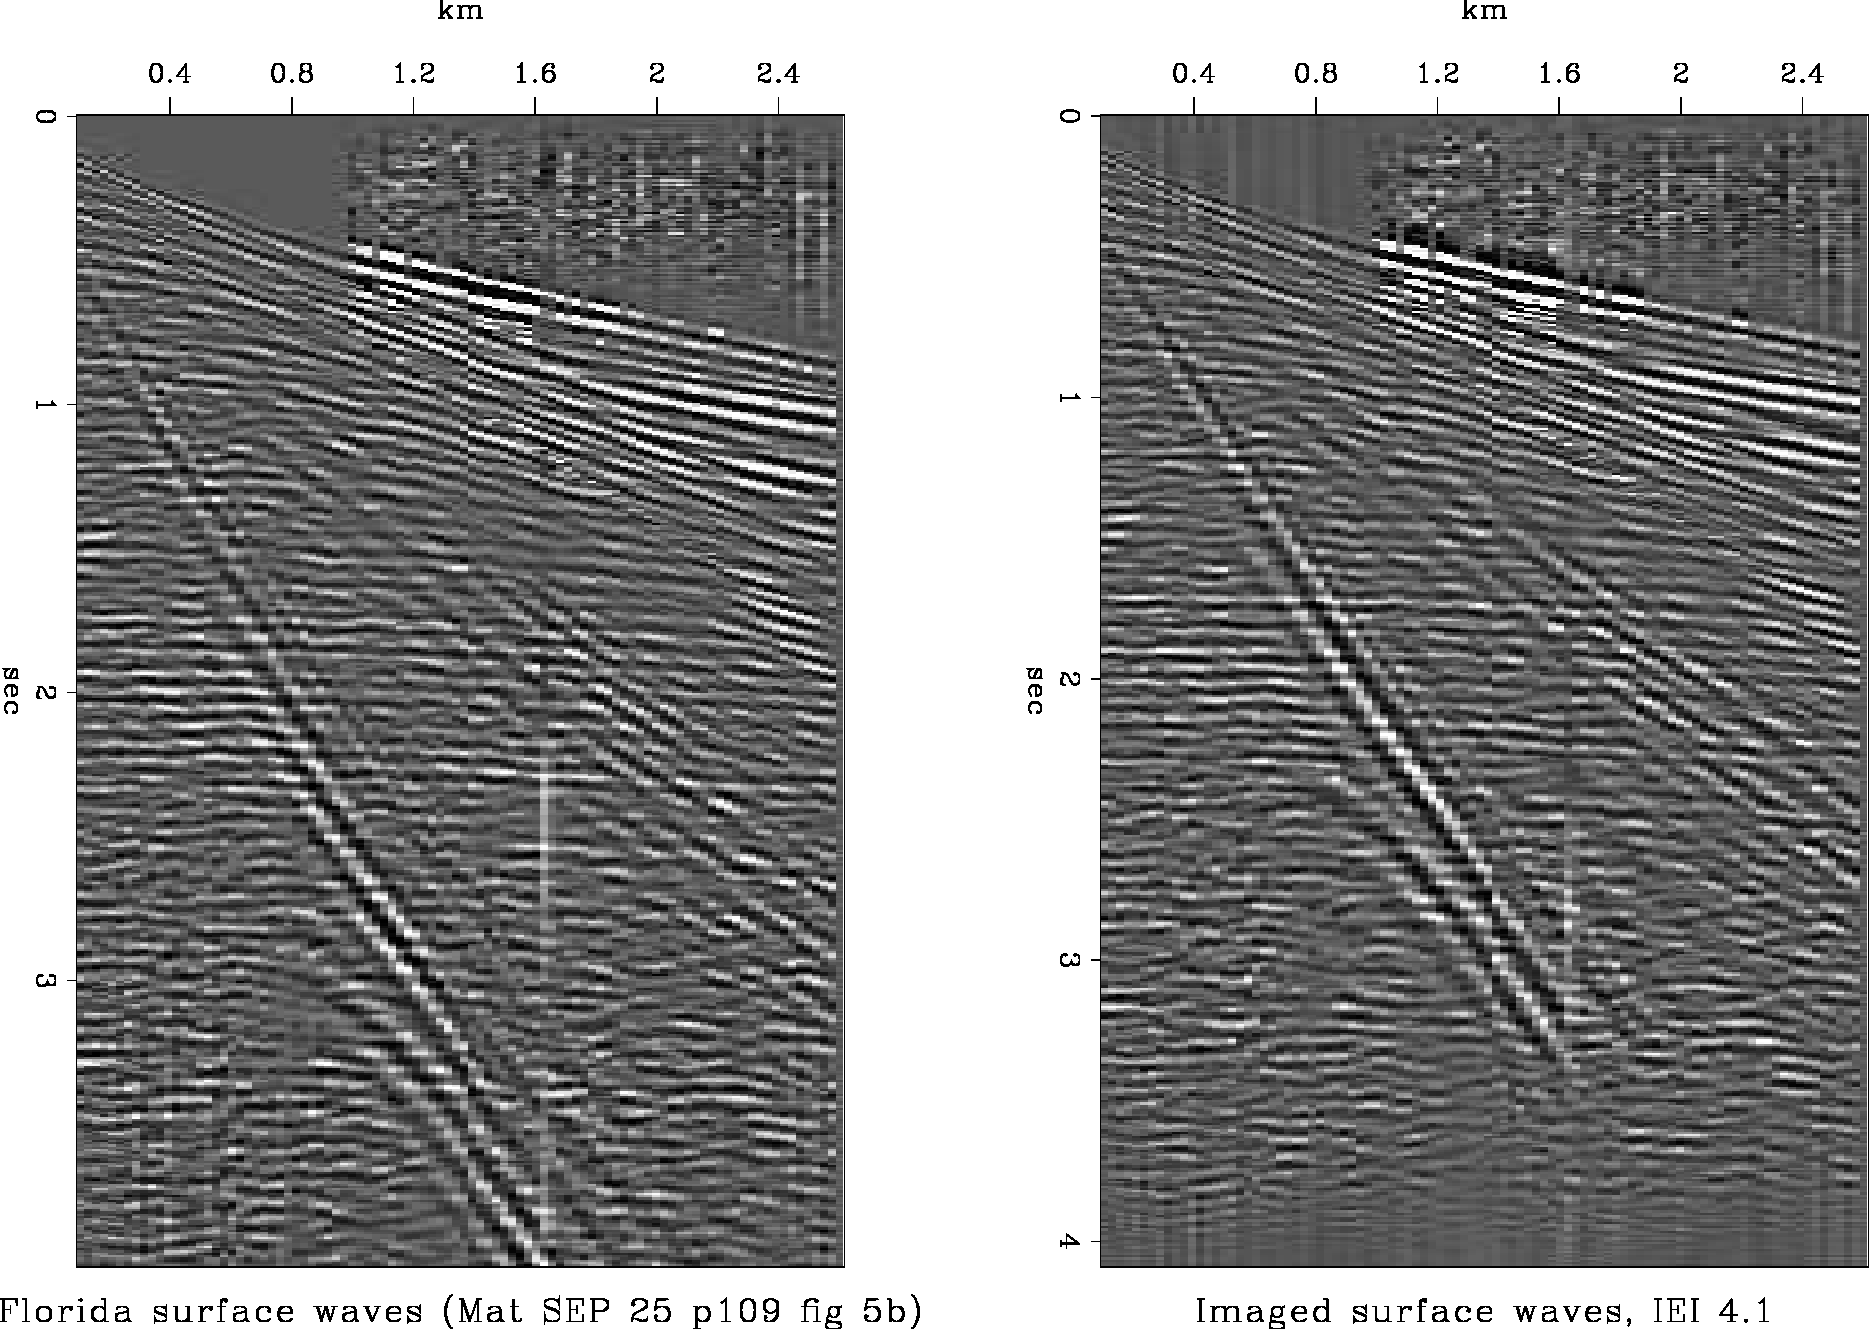
\includegraphics[width=0.65\textwidth]{dspr/sword}
% \caption[sword]{频散面波(左图)。消除频散之后(右图)。
% 图底部表示有两个波至,一是呈直线状的直达波波至,另一是双曲线的一侧,该双曲线必然是由远离测
% 线之地面上的某种物体所形成的侧反射(据Sword)}
% \label{fig:dspr/sword}
% \end{figure}
%
% \subsection{偏移剖面上的虚假半圆弧}
% \label{sec:4.1.6}
%
% 倾角滤波可用于压制多次波。\ref{sec:5.5}节将指出,多次波在一个重要方面是不同于一次波
% 的:其强度可能沿水平方向作迅速变化。对一次波,必须按绕射双曲线进行扫描偏移,对于
% 多次波,则不需知此。之所以产生这种差别,是因为对多次波经常得花费很多时间才能聚焦
% 在不规则近地表区域内。广角偏移剖面的外貌中就包含有类似这种性态的共同特征,这类剖
% 面往往表现出有许多来自所存路径直至包括来自地表面的半圆弧,这些半圆弧的出现就是警
% 告我们出了什么差错,半圆弧可能是由多次波、静校正或者无法解释的脉冲干扰所形成。在
% 许多场合下,都可以局部将它们压制掉而不蝕动到一次波。
%
% \subsection{在倾角空间内消除多次波}
% \label{sec:4.1.7}
%
% 试将对共深度点叠加结果的偏移看作是在$(\omega,k_x,z)$空间内的向下延拓。一般来
% 说,速度是随深度而增大的。当向下延拓继续迸行时,速度截止作用沿着指数衰减区的边界
% 从$(\omega,k_x)$空间中啃掉越来越多的面积(见\ref{sec:1.4}节)。超过这种截止速度的能量是不符合一
% 次波波动传播模型的,因而一遇到它就要将它压制掉。这样的噪音压制方法可能在较晚的
% 时间上导致总功率的大大下降。
%
% \subsection{倾角滤波}
% \label{sec:4.1.8}
%
% 倾角滤波能很方便地同波动外推方程结合起来。我们采用$ik_z=\epsilon-i\omega r_0$。而不是用
% $-i\omega r_0$。作初始的Muir展开(参阅\ref{sec:2.1}节,$r_0$是某个准确拟合角度的余弦)。对于15°方程,
% 我们得
% \begin{subequations}
% \begin{equation}
% ik_z^{15}v=-i\omega+\frac{v^2k_x^2}{\epsilon-i\omega(r_0+1)}
% \label{eq:ex4.1.5a}
% \end{equation}
% 对于$45^{\circ}$方程,我们有
% \begin{equation}
% ik_z^{45}v=-i\omega+\frac{v^2k_x^2}{-2i\omega+\frac{v^2k_x^2}{\epsilon-i\omega(r_0+1)}}
% \label{eq:ex4.1.5b}
% \end{equation}
% \label{eq:ex4.1.5}
% \end{subequations}
%
% 图\ref{fig:dspr/hyp15}与图\ref{fig:dspr/hyp45}表示15°和45°方程情形下具有倾角滤波参数$\epsilon$及不具有该
% 参数时的绕射双曲线。
%
% \begin{figure}[H]
% \centering
% 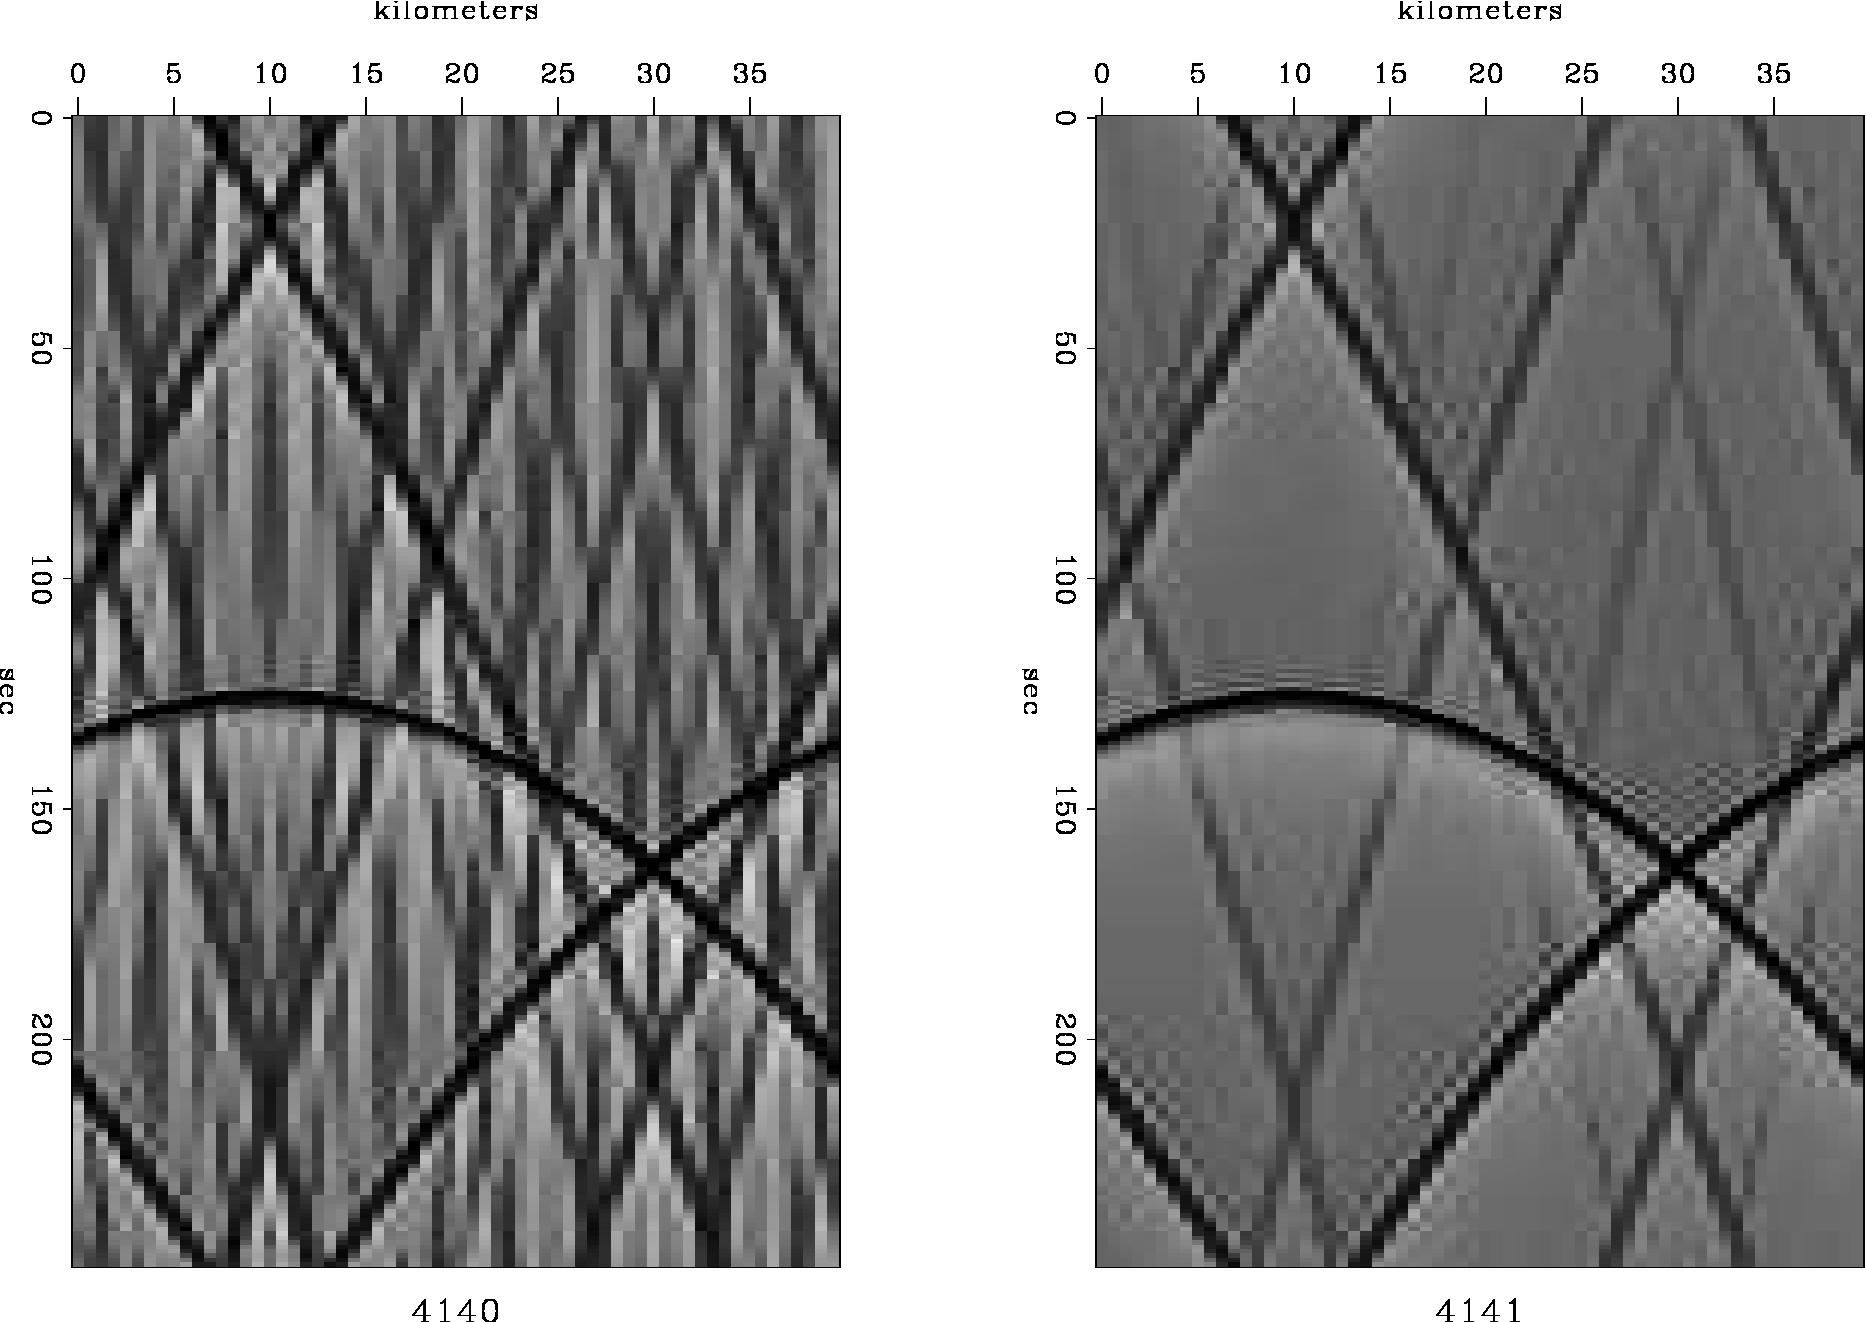
\includegraphics[width=0.65\textwidth]{dspr/hyp15}
% \caption[hyp15]{具有倾角滤波(右图)和不带倾角滤波(左图)之15°方程的绕射双曲线}
% \label{fig:dspr/hyp15}
% \end{figure}
%
% \begin{figure}[H]
% \centering
% 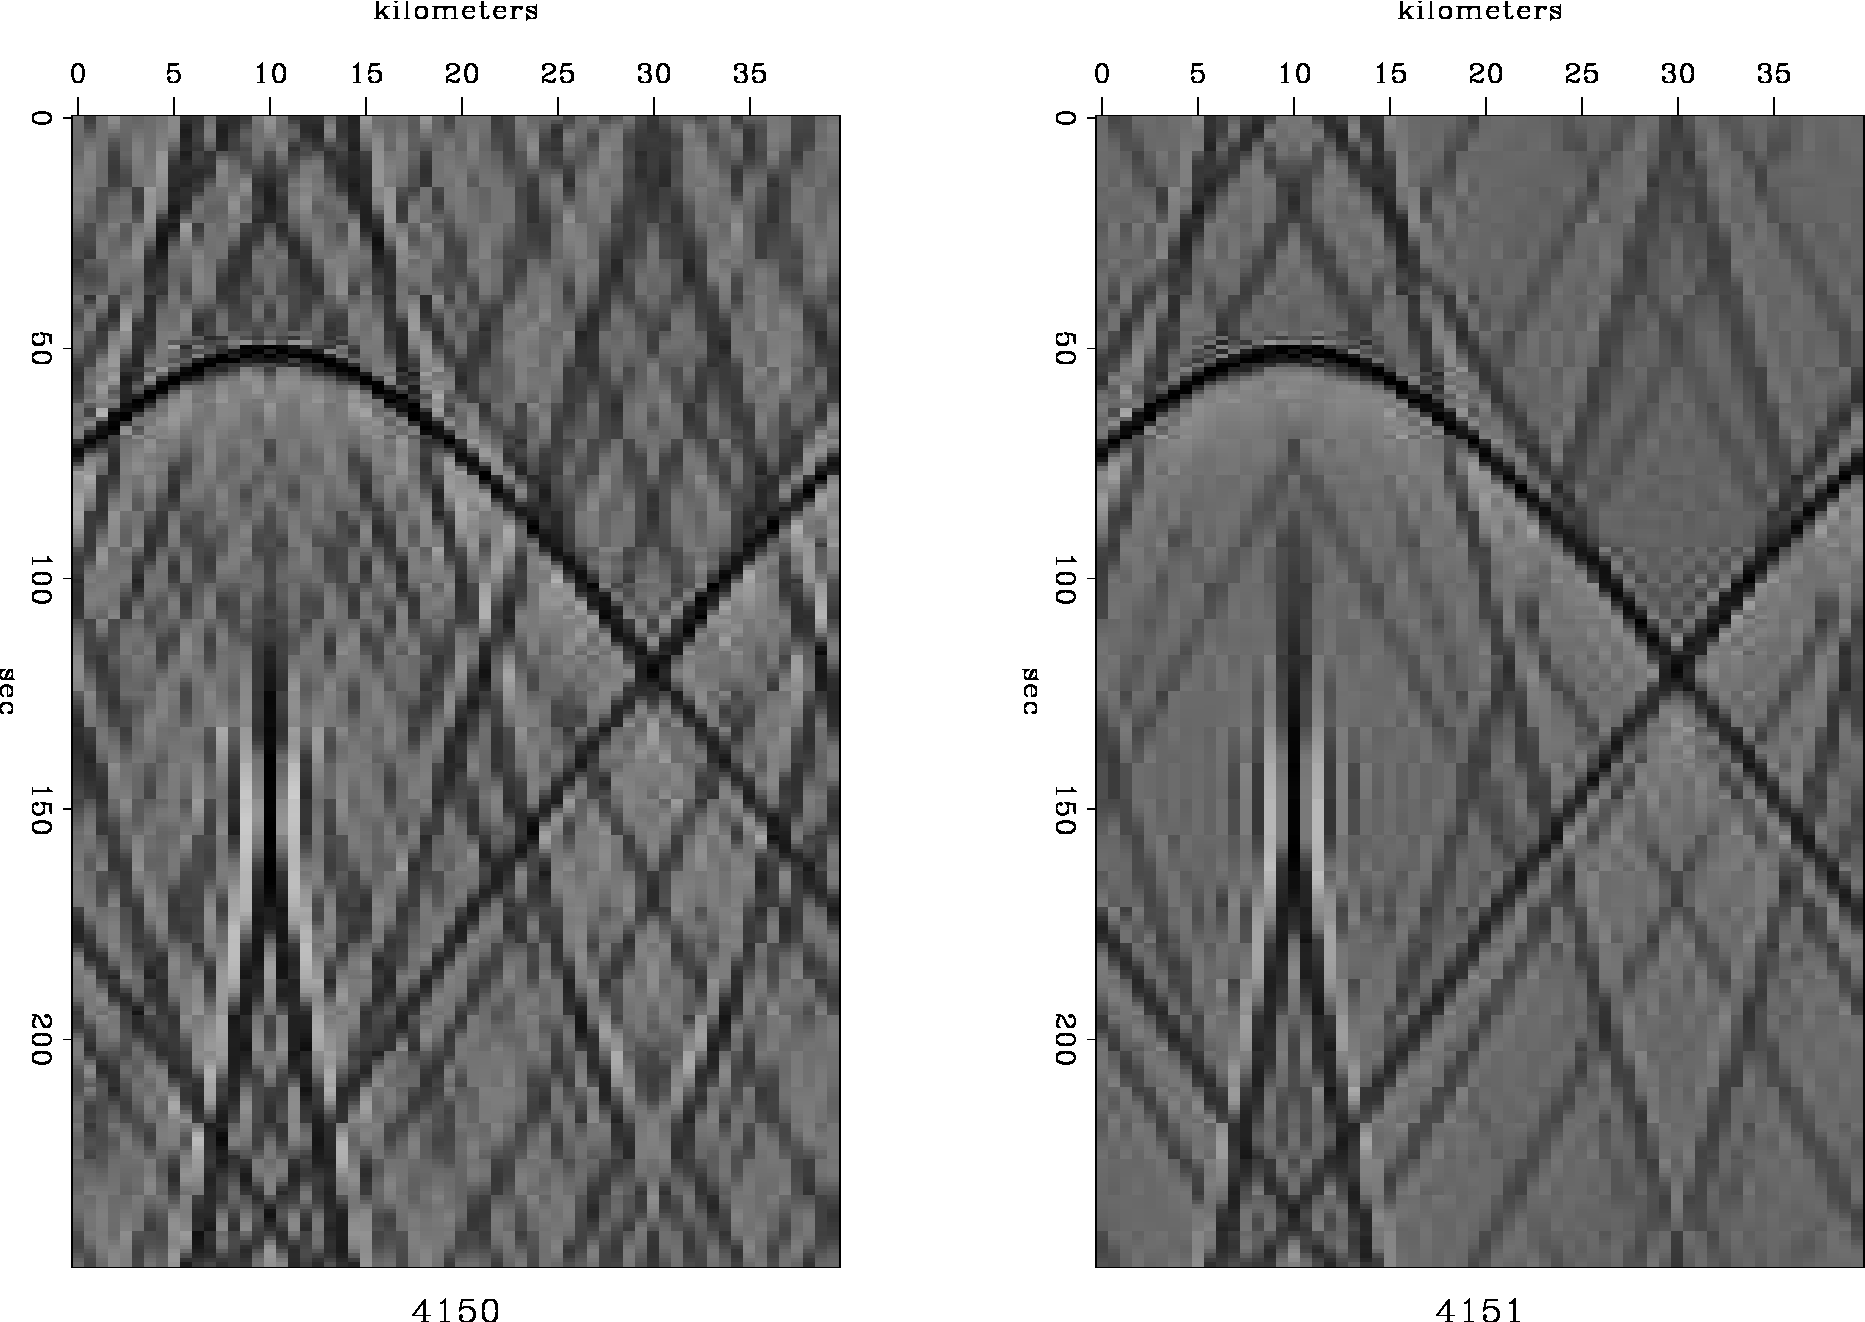
\includegraphics[width=0.65\textwidth]{dspr/hyp45}
% \caption[hyp45]{具有倾角滤波(右图)和不带倾角滤波(左图)之45°方程的绕射双曲线}
% \label{fig:dspr/hyp45}
% \end{figure}
%
% \subsection{倾角滤波资料的混杂面貌}
% \label{sec:4.1.9}
%
% 对倾角滤波经常提出的一种反对意见是:它可能把资料搞得面貌混杂。混杂的意思是指
% 各相邻记录道好像都已经加以平均,使得它们不再是独立的了。这确实是倾角滤波的一种影
% 响,而且由于反射资料水平分辨能力随时间之增大而降低,在较大时间上不可避免炮要出现
% 这种混杂。横向分辨能力之所以降低,有两个原因:第一,能量猕散引起高频成分消失;第
% 二,射绣弯曲引起深源的张角(angular aperture)减小(参阅\ref{sec:1.2}节与\ref{sec:1.5}节)。忽视这种基
% 本限制而幻想各相邻记录道应具有某种独立外貌,那是不现实的。如为了显示的目的而必需
% 避免混杂,那末,我建议消除低速相干信号生成的噪音而代之以低速非相干的高斯随机噪
% 音。许多显示装置都是在记录道间距很密时损失动态范围,而随机噪音却可能有助于恢复该
% 动态范围。
%
% \subsection{使断层显示突出}
% \label{sec:4.1.10}
%
% 经常能遇到油藏位置受断层控制的情形,但是层状反射面占优势的影响可能掩盖了表示
% 断层标志的弱绕射波,这时就需要有一种修饰性处理,能够减弱零倾角和小倾角的同相轴,
% 重点突出10度至60度的倾角范围内之同相轴,然后再将广角反射和指数衰减波能量压制掉。
% 正如频率滤波的情形一样,是不希望采用锐截止的,因为这意味着脉冲响应会很长(在空间
% 内,就是脉冲响应很宽)。
%
% \subsection{增益控制也起倾角滤波作用}
% \label{sec:4.1.11}
%
% 到达时间晚的反射都比到达时间早的反射要弱一些,所以为了显示,普通都利用时变比
% 例将数据标定。那末,究竟应当是在进行这种按比例标定之前还是在这之后完成偏移呢?答
% 案将因所感兴趣的方式而有所不同。双曲线顶部有平缓倾角,而到达时间较晚的渐近线则有
% 陡倾角,因此,放大较晚到达的信息就同放大陡倾角同相轴是完全一致的。我想,选择在比
% 例标定之前或之后进行偏移,其主要效果也就是最终显示时选择什么倾角谱的问题。过于死
% 板但正确的作法是,首先迸行偏移,其次进行比例标定,但是这会减弱倾斜同相轴和断层的
% 信息。而首先进行比例标定,其次进行偏移,则所得结果就比较好一点。后面这种作法有一
% 个附带的好处,就是采用短字长整数来存贮已经标定过的值,你可以节省计算机内存。在
% 我的先驱性工作中,我曾采用16位整数存贮,计算与局部存贮采用32位浮点算法。我看很少
% 有理由要采用现今一般所利用的32位存贮,我们进行记录道之间的内插还不可能达到4位的
% 精度。
%
% \subsection{是非相干性还是滤波所产生的压制作用}
% \label{sec:4.1.12}
%
% 根据修饰性效果来判断所设想的非修饰性处理,是有潜在危险的。我就曾碰到过这么一
% 次。采用的处理是叠前偏移,记录上很清晰的最陡同相轴之相对强度据信是断层面反射的特
% 征,但是谁知道即使是增益控制也可能会影响倾角谱!我希望叠前偏移处理能起作用的是正
% 确消除共深度点叠加对陡倾角同相轴的某种截止影响。也许事实确是如此,但是我怎么才能
% 知道到底是这种猜想正在实现呢,还是空间滤波作用偶然地正在增强倾斜同相轴呢?
%
% \subsection{偏移之前的空间比例标定}
% \label{sec:4.1.13}
%
% 在偏移之前对时间轴进行比例标定,可以有好处,那末对空间坐标轴进行比例标定又会
% 怎么样呢?称为自动增益控制(AGC
% )的传统标定方法是沿某种时窗对数据的包络(或者
% 它的平方或绝对值)进行平滑处理,导出一个比例因子。这样的比例标定可以逐道迅速变
% 化。因此担心比例函数的横向跃变也许会形成绕射是有道理的。另一方面,比例逐道迅速跃
% 变,确实也可能是有充分原因的。为采集陆地资料而采用的炮点和检波器逋常都有可变的强
% 度和耦合作用,而这些问题是会影晌到整个记录道的。
%
% 必须找到一个既遵守物理规律又照顾到统计规律的模型。我建议允许增益是缓慢时变
% 的,而炮点和检波点则具有任意可变强度,但是我也推荐把脉冲看成是地层确实能够聚焦的
% 证据。例如,采用下列滤波:
% \begin{equation}
% 1-\frac{\omega^2}{1+\alpha\omega^2}\frac{k_x^2}{1+\beta k_x^2}
% \label{eq:ex4.1.6}
% \end{equation}
% 对标定的包络进行平滑,就可以实现利用这种模型的数据处理。滤波截止参量为$\alpha$与$\beta$。当标
% 定的包络用这种滤波加以平滑后,它就不再是同时随时间$t$和空间坐标$x$二者而迅速变化
% 了,尽管它还可能随这一个或者那一个而变化。利用三对角线算法,可以很节省时间地实现
% 式\ref{eq:ex4.1.6}这种滤波处理。
%
% \subsection{指数比例标定}
% \label{sec:4.1.14}
%
% 指数比例函数具有某些理想的数学性质。取时间函数$a_t$的$Z$变换:
% \begin{equation}
% A(Z)=a_0+a_1Z+a_2Z^2+......
% \label{eq:ex4.1.7}
% \end{equation}
% 指数增益时间函数按下式定义
% \begin{equation}
% \uparrow A(Z)=a_0+a_1e^\alpha Z+a_2e^{2\alpha} Z^2+......
% \label{eq:ex4.1.8}
% \end{equation}
% 箭头符号$\uparrow$表示指数增益,从数学上说,$\uparrow$的意思就是用$e^\alpha Z$代替Z。多项式乘法相当于诸
% 系数之褶积
% \begin{equation}
% C(Z)=A(Z)B(Z)
% \label{eq:ex4.1.9}
% \end{equation}
% 根据直接代入的办法,得
% \begin{equation}
% \uparrow C=(\uparrow A)(\uparrow B)
% \label{eq:ex4.1.10}
% \end{equation}
% 这意味着可以在褶积之前或之后完成指数增益。根据Fourier变换理论你会想起,一个时间
% 函数用一个衰减指数$\exp(-\alpha t)$来乘,在变换域内就等价于用$-i\omega+\alpha$
% 来代替$-i\omega$。
%
% 现在,在某个固定$z$值和某个固定L值的具体情形下来讨论向下延拓算子$\exp(ik_zz)$
% 这时该算子变成了频率$\omega$的一个函数,在时间域内能将它表示为滤波函数心。在偏移的时
% 候,双曲线两侧翼是向上移动的,所以心应是反时间因果性滤波算子(anticausal),以下
% 式表示这种性质
% \begin{equation}
% A(Z)=a_0+a_{-1}\frac{1}{Z}+a_{-2}\frac{1}{Z^2}+......
% \label{eq:ex4.1.11}
% \end{equation}
% 复变量Z的大值负幂均同双曲线两侧翼有关,指数型提高Z的正幂系数是同减小负幂有联系
% 的---所以$\uparrow A$是带有被削弱了尾部的函数A---
% 因而有助于使双曲线两翼衰减而不是移动
% 它们,因此就能把$\uparrow A$说成是具有粘滞性的。
%
% 从纯粹物理的观点看,像增益控制和倾角滤波这类修饰性函数,应该是在处理之后,比
% 方说,在完成$\uparrow(AB)$之后再采用。但是$\uparrow(AB)$等价于$(\uparrow A)(\uparrow B)$、即等价于先采用修饰
% 性函数后作褶积姓理,而且像$(\uparrow A)(\uparrow B)$这种运算还相当于是对已作指数增益的数据采用
% 粘滞性算子。在实践中,通常都是忘掉粘滞性而形成$A(\uparrow B)$这种运算,这样作或许是因为
% 考虑到倾斜同相轴携带有比平缓同相轴更多的信息。
%
% \subsection{代换算子}
% \label{sec:4.1.15}
%
% 算子$\uparrow$在前面业已定义为代换$Z\rightarrow Ze^\alpha$,这种算子的主要性质是;如果$C=AB$,则
% $\uparrow C= (\uparrow A)(\uparrow B)$。这种性质对于变量Z时任何代数替换都应是共有的性质,而非仅对指数
% 增益一种情形才成立。要达到时间轴拉伸或压缩的结果,可以采用另一种简单代换,例如,
% 用Z\textsuperscript{2}代替Z,就是把时间轴拉伸一倍。还有意义比前两种更深刻的另外一种代换,即以耗散
% 算子$(-i\omega)^\gamma$代替恒定Q值。各种代换可列成下表:
% \begin{table}[!ht]
% \centering
% \ttfamily
% \small
% \begin{tabularx}{\textwidth}{Y|Y}
% \hline
% \multicolumn{2}{Y}{Z变换变量Z的代换(均保持$C(Z)=A(Z)B(Z)$形式)} \\
% \hline
% 指数增长& $Z\rightarrow Ze^{\alpha}, (i\omega\rightarrow i\omega+\alpha)$\\
% \hline
% 时间扩展$(\alpha >1)$&$Z\rightarrow Z^{\alpha}$\\
% \hline
% (逆)恒定Q值耗散&$-i\omega \rightarrow (-i\omega)^\gamma$ \\
% \hline
% \end{tabularx}
% \end{table}
% \subsection{习题}
% \label{sec:4.1.16}
%
% \begin{enumerate}
% \item
%   利用积分表证明:地震震源具有形式为$\mid \omega\mid^\beta$之谱,则意味着发散校正应为$t^{2+\beta}$。
% \item
%   设$t^2$为野外剖面的一个适当的发散校正因子,试问:对共深度点叠加应该应用什
%   么样的发散校正?
% \item
%   试问应如何改动t\textsuperscript{2}校正使之适用于旅行时间深度为$t_0$之海水层?设海水层的Q值
%   为无限大。
% \item
%   考虑震源谱为$e^{-\beta\mid\omega\mid}$的情形,试问应如何改变$t^2$校正?
% \end{enumerate}
